\chapter{Appendix}
\label{cha:appendix}

\section{Accuracy Evaluation}

\begin{table}[htpb]
    \centering
    \scriptsize
    \begin{tabular}{lr|lr|lr|lr}
        \toprule
        Project & Points & Project & Points & Project & Points & Project & Points \\
        \midrule
        K6\_S01 & 30 & K6\_S10 & 22 & K7\_S02 & 19 & K7\_S14 & 24 \\
        K6\_S02 & 15 & K6\_S15 & 10 & K7\_S03 & 14 & K7\_S15 & 25 \\
        K6\_S03 & 11 & K6\_S17 & 2  & K7\_S04 & 12 & K7\_S16 & 19 \\
        K6\_S05 & 23 & K6\_S18 & 27 & K7\_S05 & 22 & K7\_S17 & 29 \\
        K6\_S06 & 30 & K6\_S19 & 25 & K7\_S06 & 20 & K7\_S18 & 19 \\
        K6\_S11 & 8  & K6\_S20 & 30 & K7\_S07 & 20 & K7\_S19 & 22 \\
        K6\_S12 & 6  & K6\_S29 & 12 & K7\_S08 & 21 & K7\_S20 & 9  \\
        K6\_S13 & 8  & K6\_S30 & 20 & K7\_S10 & 25 & K7\_S24 & 2  \\
        K6\_S14 & 4  & K6\_S31 & 16 & K7\_S11 & 8  & K7\_S26 & 22 \\
        K6\_S16 & 2  & K6\_S33 & 20 & K7\_S12 & 27 & K7\_S27 & 8  \\
        K6\_S27 & 4  \\
        \bottomrule
    \end{tabular}
    \caption{Manual scores of each project in P1}
    \label{tab:manual_scores_of_each_project}
\end{table}

\section{Inconsistency Evaluation}
\label{sec:inconsistency_evaluation}

\begin{table}
    \setlength{\tabcolsep}{0.2em}
    \tiny
    \centering
    \begin{tabular}{l|rrrrrrrrrrrrrrrrrrrrrrrrrrrr}
        \toprule
        & 01 & 02 & 03 & 04 & 05 & 06 & 07 & 08 & 09 & 10 & 11 & 12 & 13 & 14 & 15 & 16 & 17 & 18 & 19 & 20 & 21 & 22 & 23 & 24 & 25 & 26 & 27 & 28 \\
        \midrule
        K6\_S02 & 0 & 0 & 0 & 0 & 0 & 0 & 0 & 0 & 0 & 0 & 0 & 0 & 0 & \textbf{1} & \textbf{1} & 0 & 0 & 0 & 0 & 0 & 0 & 0 & \textbf{1} & 0 & 0 & 0 & 0 & 0 \\
        K6\_S03 & 0 & 0 & 0 & 0 & 0 & 0 & 0 & \textbf{1} & 0 & 0 & 0 & 0 & \textbf{1} & \textbf{1} & \textbf{1} & 0 & \textbf{1} & 0 & 0 & 0 & 0 & 0 & 0 & 0 & 0 & 0 & 0 & 0 \\
        K6\_S05 & 0 & 0 & 0 & 0 & 0 & 0 & 0 & 0 & 0 & 0 & 0 & 0 & 0 & 0 & 0 & 0 & 0 & 0 & 0 & 0 & 0 & 0 & 0 & 0 & 0 & 0 & 0 & 0 \\
        K6\_S10 & 0 & 0 & 0 & 0 & 0 & 0 & 0 & 0 & 0 & 0 & 0 & 0 & \textbf{1} & \textbf{1} & 0 & 0 & 0 & 0 & 0 & 0 & 0 & 0 & \textbf{1} & 0 & 0 & 0 & 0 & 0 \\
        K6\_S11 & 0 & 0 & 0 & 0 & 0 & 0 & 0 & 0 & 0 & 0 & 0 & 0 & 0 & 0 & 0 & 0 & 0 & 0 & \textbf{1} & 0 & 0 & 0 & 0 & 0 & 0 & 0 & 0 & 0 \\
        K6\_S13 & 0 & 0 & 0 & 0 & 0 & 0 & 0 & 0 & 0 & 0 & 0 & 0 & 0 & 0 & 0 & 0 & 0 & 0 & 0 & 0 & 0 & 0 & 0 & 0 & 0 & 0 & 0 & 0 \\
        K6\_S15 & 0 & 0 & 0 & 0 & 0 & 0 & 0 & 0 & 0 & 0 & 0 & 0 & 0 & 0 & 0 & 0 & 0 & 0 & 0 & 0 & 0 & 0 & 0 & 0 & 0 & 0 & 0 & 0 \\
        K6\_S16 & 0 & 0 & 0 & 0 & 0 & 0 & 0 & 0 & 0 & 0 & 0 & 0 & 0 & 0 & 0 & 0 & 0 & 0 & 0 & 0 & 0 & 0 & 0 & 0 & 0 & 0 & 0 & 0 \\
        K6\_S18 & 0 & 0 & 0 & 0 & 0 & 0 & 0 & 0 & 0 & 0 & 0 & 0 & 0 & 0 & 0 & 0 & 0 & 0 & 0 & 0 & 0 & 0 & 0 & 0 & 0 & 0 & 0 & 0 \\
        K6\_S19 & 0 & 0 & 0 & 0 & 0 & 0 & 0 & 0 & 0 & 0 & 0 & 0 & 0 & 0 & 0 & 0 & 0 & 0 & 0 & 0 & 0 & 0 & \textbf{1} & 0 & 0 & 0 & \textbf{1} & 0 \\
        K6\_S27 & 0 & 0 & 0 & 0 & 0 & 0 & 0 & 0 & 0 & 0 & 0 & 0 & 0 & 0 & 0 & 0 & 0 & 0 & 0 & 0 & 0 & 0 & 0 & 0 & 0 & 0 & 0 & 0 \\
        K6\_S29 & 0 & 0 & 0 & 0 & 0 & 0 & 0 & 0 & 0 & 0 & 0 & 0 & 0 & 0 & 0 & 0 & 0 & 0 & 0 & 0 & 0 & 0 & 0 & 0 & 0 & 0 & 0 & 0 \\
        K6\_S30 & 0 & 0 & 0 & 0 & 0 & 0 & 0 & 0 & 0 & 0 & 0 & 0 & 0 & 0 & 0 & 0 & 0 & 0 & 0 & 0 & 0 & 0 & 0 & 0 & 0 & 0 & 0 & 0 \\
        K6\_S31 & 0 & 0 & 0 & 0 & 0 & 0 & 0 & 0 & 0 & 0 & 0 & 0 & 0 & 0 & 0 & 0 & 0 & 0 & 0 & 0 & 0 & 0 & 0 & 0 & 0 & 0 & 0 & 0 \\
        K6\_S33 & 0 & 0 & 0 & 0 & 0 & 0 & 0 & \textbf{1} & \textbf{1} & 0 & 0 & 0 & 0 & 0 & 0 & 0 & 0 & 0 & 0 & 0 & 0 & 0 & 0 & 0 & 0 & 0 & 0 & 0 \\
        K7\_S02 & 0 & 0 & 0 & 0 & 0 & 0 & 0 & 0 & 0 & 0 & 0 & 0 & 0 & 0 & 0 & 0 & 0 & 0 & 0 & 0 & \textbf{1} & 0 & 0 & 0 & 0 & 0 & 0 & 0 \\
        K7\_S03 & 0 & 0 & 0 & 0 & 0 & 0 & 0 & 0 & 0 & 0 & 0 & 0 & \textbf{1} & \textbf{1} & 0 & 0 & \textbf{1} & 0 & 0 & 0 & 0 & 0 & 0 & 0 & 0 & 0 & 0 & 0 \\
        K7\_S04 & 0 & 0 & 0 & 0 & 0 & 0 & 0 & 0 & 0 & 0 & 0 & 0 & 0 & 0 & 0 & 0 & 0 & 0 & 0 & 0 & 0 & 0 & 0 & 0 & 0 & 0 & 0 & 0 \\
        K7\_S05 & 0 & 0 & 0 & 0 & 0 & 0 & 0 & 0 & 0 & 0 & 0 & 0 & 0 & 0 & 0 & 0 & 0 & 0 & 0 & 0 & 0 & 0 & 0 & 0 & 0 & 0 & 0 & 0 \\
        K7\_S06 & 0 & 0 & 0 & 0 & 0 & 0 & 0 & 0 & 0 & 0 & 0 & 0 & 0 & 0 & 0 & 0 & 0 & 0 & 0 & 0 & 0 & 0 & 0 & 0 & 0 & 0 & 0 & 0 \\
        K7\_S07 & 0 & 0 & 0 & 0 & 0 & 0 & 0 & 0 & 0 & 0 & 0 & 0 & \textbf{1} & 0 & \textbf{1} & 0 & \textbf{1} & 0 & 0 & 0 & 0 & 0 & \textbf{1} & 0 & 0 & 0 & 0 & 0 \\
        K7\_S08 & 0 & 0 & 0 & 0 & 0 & 0 & 0 & 0 & 0 & 0 & 0 & 0 & 0 & 0 & 0 & 0 & 0 & 0 & 0 & 0 & 0 & 0 & 0 & 0 & 0 & 0 & 0 & 0 \\
        K7\_S10 & 0 & 0 & 0 & 0 & 0 & 0 & 0 & 0 & 0 & 0 & 0 & 0 & 0 & 0 & 0 & 0 & 0 & 0 & 0 & 0 & \textbf{1} & 0 & 0 & 0 & 0 & 0 & 0 & 0 \\
        K7\_S11 & 0 & 0 & 0 & 0 & 0 & 0 & 0 & 0 & 0 & 0 & 0 & 0 & 0 & 0 & 0 & 0 & 0 & 0 & 0 & 0 & 0 & 0 & 0 & 0 & 0 & 0 & 0 & 0 \\
        K7\_S12 & 0 & 0 & 0 & 0 & 0 & 0 & 0 & 0 & 0 & 0 & 0 & 0 & 0 & \textbf{1} & 0 & 0 & 0 & 0 & 0 & 0 & 0 & 0 & 0 & 0 & 0 & 0 & 0 & 0 \\
        K7\_S14 & 0 & 0 & 0 & 0 & 0 & 0 & 0 & 0 & 0 & 0 & 0 & 0 & 0 & 0 & 0 & 0 & 0 & 0 & 0 & 0 & 0 & 0 & 0 & 0 & 0 & 0 & 0 & 0 \\
        K7\_S15 & 0 & 0 & 0 & 0 & 0 & 0 & 0 & 0 & 0 & 0 & 0 & 0 & 0 & 0 & 0 & 0 & 0 & 0 & 0 & 0 & 0 & 0 & 0 & \textbf{1} & 0 & 0 & 0 & 0 \\
        K7\_S16 & 0 & 0 & 0 & \textbf{1} & \textbf{1} & 0 & 0 & 0 & 0 & 0 & 0 & 0 & 0 & 0 & 0 & 0 & 0 & 0 & 0 & 0 & 0 & 0 & 0 & 0 & 0 & 0 & 0 & 0 \\
        K7\_S17 & 0 & 0 & 0 & 0 & 0 & 0 & 0 & 0 & 0 & 0 & 0 & 0 & 0 & 0 & 0 & 0 & 0 & 0 & \textbf{1} & 0 & \textbf{1} & 0 & 0 & \textbf{1} & 0 & 0 & 0 & 0 \\
        K7\_S19 & 0 & 0 & 0 & 0 & 0 & 0 & 0 & 0 & 0 & 0 & 0 & 0 & 0 & 0 & 0 & 0 & 0 & 0 & 0 & 0 & 0 & 0 & \textbf{1} & 0 & 0 & 0 & 0 & 0 \\
        K7\_S20 & 0 & 0 & 0 & 0 & 0 & 0 & 0 & 0 & 0 & 0 & 0 & 0 & 0 & 0 & 0 & 0 & 0 & 0 & 0 & 0 & 0 & \textbf{1} & 0 & 0 & 0 & 0 & 0 & 0 \\
        K7\_S26 & 0 & 0 & 0 & 0 & 0 & 0 & 0 & 0 & 0 & 0 & 0 & 0 & 0 & 0 & 0 & 0 & 0 & 0 & 0 & 0 & 0 & 0 & 0 & \textbf{1} & 0 & 0 & 0 & 0 \\
        \bottomrule
    \end{tabular}
    \caption{Inconsistency matrix for test suite T1 (normal tests)}
    \label{tab:inconsistencies_matrix_normal}
    \setlength{\tabcolsep}{\defaulttabcolsep}
    \mnote{TODO: update}
\end{table}

\begin{table}
    \setlength{\tabcolsep}{0.2em}
    \tiny
    \centering
    \begin{tabular}{l|rrrrrrrrrrrrrrrrrrrrrrrrrrrr}
        \toprule
        & 01 & 02 & 03 & 04 & 05 & 06 & 07 & 08 & 09 & 10 & 11 & 12 & 13 & 14 & 15 & 16 & 17 & 18 & 19 & 20 & 21 & 22 & 23 & 24 & 25 & 26 & 27 & 28 \\
        \midrule
        K6\_S02 & 0 & 0 & 0 & 0 & 0 & 0 & 0 & 0 & 0 & 0 & 0 & 0 & 0 & \textbf{1} & \textbf{1} & 0 & 0 & 0 & 0 & 0 & 0 & 0 & \textbf{1} & 0 & 0 & 0 & 0 & 0 \\
        K6\_S03 & 0 & 0 & 0 & 0 & 0 & 0 & 0 & \textbf{1} & 0 & 0 & 0 & 0 & \textbf{1} & \textbf{1} & \textbf{1} & 0 & \textbf{1} & 0 & 0 & 0 & 0 & 0 & 0 & 0 & 0 & 0 & 0 & 0 \\
        K6\_S05 & 0 & 0 & 0 & 0 & 0 & 0 & 0 & 0 & 0 & 0 & 0 & 0 & 0 & 0 & 0 & 0 & 0 & 0 & 0 & 0 & 0 & 0 & 0 & 0 & 0 & 0 & 0 & 0 \\
        K6\_S10 & 0 & 0 & 0 & 0 & 0 & 0 & 0 & 0 & 0 & 0 & 0 & 0 & \textbf{1} & \textbf{1} & 0 & 0 & 0 & 0 & 0 & 0 & 0 & 0 & \textbf{1} & 0 & 0 & 0 & 0 & 0 \\
        K6\_S11 & 0 & 0 & 0 & 0 & 0 & 0 & 0 & 0 & 0 & 0 & 0 & 0 & 0 & 0 & 0 & 0 & 0 & 0 & \textbf{1} & 0 & 0 & 0 & 0 & 0 & 0 & 0 & 0 & 0 \\
        K6\_S13 & 0 & 0 & 0 & 0 & 0 & 0 & 0 & 0 & 0 & 0 & 0 & 0 & 0 & 0 & 0 & 0 & 0 & 0 & 0 & 0 & 0 & 0 & 0 & 0 & 0 & 0 & 0 & 0 \\
        K6\_S15 & 0 & 0 & 0 & 0 & 0 & 0 & 0 & 0 & 0 & 0 & 0 & 0 & 0 & 0 & 0 & 0 & 0 & 0 & 0 & 0 & 0 & 0 & 0 & 0 & 0 & 0 & 0 & 0 \\
        K6\_S16 & 0 & 0 & 0 & 0 & 0 & 0 & 0 & 0 & 0 & 0 & 0 & 0 & 0 & 0 & 0 & 0 & 0 & 0 & 0 & 0 & 0 & 0 & 0 & 0 & 0 & 0 & 0 & 0 \\
        K6\_S18 & 0 & 0 & 0 & 0 & 0 & 0 & 0 & 0 & 0 & 0 & 0 & 0 & 0 & 0 & 0 & 0 & 0 & 0 & 0 & 0 & 0 & 0 & 0 & 0 & 0 & 0 & 0 & 0 \\
        K6\_S19 & 0 & 0 & 0 & 0 & 0 & 0 & 0 & 0 & 0 & 0 & 0 & 0 & 0 & 0 & 0 & 0 & 0 & 0 & 0 & 0 & 0 & 0 & \textbf{1} & 0 & 0 & 0 & \textbf{1} & 0 \\
        K6\_S27 & 0 & 0 & 0 & 0 & 0 & 0 & 0 & 0 & 0 & 0 & 0 & 0 & 0 & 0 & 0 & 0 & 0 & 0 & 0 & 0 & 0 & 0 & 0 & 0 & 0 & 0 & 0 & 0 \\
        K6\_S29 & 0 & 0 & 0 & 0 & 0 & 0 & 0 & 0 & 0 & 0 & 0 & 0 & 0 & 0 & 0 & 0 & 0 & 0 & 0 & 0 & 0 & 0 & 0 & 0 & 0 & 0 & 0 & 0 \\
        K6\_S30 & 0 & 0 & 0 & 0 & 0 & 0 & 0 & 0 & 0 & 0 & 0 & 0 & 0 & 0 & 0 & 0 & 0 & 0 & 0 & 0 & 0 & 0 & 0 & 0 & 0 & 0 & 0 & 0 \\
        K6\_S31 & 0 & 0 & 0 & 0 & 0 & 0 & 0 & 0 & 0 & 0 & 0 & 0 & 0 & 0 & 0 & 0 & 0 & 0 & 0 & 0 & 0 & 0 & 0 & 0 & 0 & 0 & 0 & 0 \\
        K6\_S33 & 0 & 0 & 0 & 0 & 0 & 0 & 0 & \textbf{1} & \textbf{1} & 0 & 0 & 0 & 0 & 0 & 0 & 0 & 0 & 0 & 0 & 0 & 0 & 0 & 0 & 0 & 0 & 0 & 0 & 0 \\
        K7\_S02 & 0 & 0 & 0 & 0 & 0 & 0 & 0 & 0 & 0 & 0 & 0 & 0 & 0 & 0 & 0 & 0 & 0 & 0 & 0 & 0 & \textbf{1} & 0 & 0 & 0 & 0 & 0 & 0 & 0 \\
        K7\_S03 & 0 & 0 & 0 & 0 & 0 & 0 & 0 & 0 & 0 & 0 & 0 & 0 & \textbf{1} & \textbf{1} & 0 & 0 & \textbf{1} & 0 & 0 & 0 & 0 & 0 & 0 & 0 & 0 & 0 & 0 & 0 \\
        K7\_S04 & 0 & 0 & 0 & 0 & 0 & 0 & 0 & 0 & 0 & 0 & 0 & 0 & 0 & 0 & 0 & 0 & 0 & 0 & 0 & 0 & 0 & 0 & 0 & 0 & 0 & 0 & 0 & 0 \\
        K7\_S05 & 0 & 0 & 0 & 0 & 0 & 0 & 0 & 0 & 0 & 0 & 0 & 0 & 0 & 0 & 0 & 0 & 0 & 0 & 0 & 0 & 0 & 0 & 0 & 0 & 0 & 0 & 0 & 0 \\
        K7\_S06 & 0 & 0 & 0 & 0 & 0 & 0 & 0 & 0 & 0 & 0 & 0 & 0 & 0 & 0 & 0 & 0 & 0 & 0 & 0 & 0 & 0 & 0 & 0 & 0 & 0 & 0 & 0 & 0 \\
        K7\_S07 & 0 & 0 & 0 & 0 & 0 & 0 & 0 & 0 & 0 & 0 & 0 & 0 & \textbf{1} & 0 & \textbf{1} & 0 & \textbf{1} & 0 & 0 & 0 & 0 & 0 & \textbf{1} & 0 & 0 & 0 & 0 & 0 \\
        K7\_S08 & 0 & 0 & 0 & 0 & 0 & 0 & 0 & 0 & 0 & 0 & 0 & 0 & 0 & 0 & 0 & 0 & 0 & 0 & 0 & 0 & 0 & 0 & 0 & 0 & 0 & 0 & 0 & 0 \\
        K7\_S10 & 0 & 0 & 0 & 0 & 0 & 0 & 0 & 0 & 0 & 0 & 0 & 0 & 0 & 0 & 0 & 0 & 0 & 0 & 0 & 0 & \textbf{1} & 0 & 0 & 0 & 0 & 0 & 0 & 0 \\
        K7\_S11 & 0 & 0 & 0 & 0 & 0 & 0 & 0 & 0 & 0 & 0 & 0 & 0 & 0 & 0 & 0 & 0 & 0 & 0 & 0 & 0 & 0 & 0 & 0 & 0 & 0 & 0 & 0 & 0 \\
        K7\_S12 & 0 & 0 & 0 & 0 & 0 & 0 & 0 & 0 & 0 & 0 & 0 & 0 & 0 & \textbf{1} & 0 & 0 & 0 & 0 & 0 & 0 & 0 & 0 & 0 & 0 & 0 & 0 & 0 & 0 \\
        K7\_S14 & 0 & 0 & 0 & 0 & 0 & 0 & 0 & 0 & 0 & 0 & 0 & 0 & 0 & 0 & 0 & 0 & 0 & 0 & 0 & 0 & 0 & 0 & 0 & 0 & 0 & 0 & 0 & 0 \\
        K7\_S15 & 0 & 0 & 0 & 0 & 0 & 0 & 0 & 0 & 0 & 0 & 0 & 0 & 0 & 0 & 0 & 0 & 0 & 0 & 0 & 0 & 0 & 0 & 0 & \textbf{1} & 0 & 0 & 0 & 0 \\
        K7\_S16 & 0 & 0 & 0 & \textbf{1} & \textbf{1} & 0 & 0 & 0 & 0 & 0 & 0 & 0 & 0 & 0 & 0 & 0 & 0 & 0 & 0 & 0 & 0 & 0 & 0 & 0 & 0 & 0 & 0 & 0 \\
        K7\_S17 & 0 & 0 & 0 & 0 & 0 & 0 & 0 & 0 & 0 & 0 & 0 & 0 & 0 & 0 & 0 & 0 & 0 & 0 & \textbf{1} & 0 & \textbf{1} & 0 & 0 & \textbf{1} & 0 & 0 & 0 & 0 \\
        K7\_S19 & 0 & 0 & 0 & 0 & 0 & 0 & 0 & 0 & 0 & 0 & 0 & 0 & 0 & 0 & 0 & 0 & 0 & 0 & 0 & 0 & 0 & 0 & \textbf{1} & 0 & 0 & 0 & 0 & 0 \\
        K7\_S20 & 0 & 0 & 0 & 0 & 0 & 0 & 0 & 0 & 0 & 0 & 0 & 0 & 0 & 0 & 0 & 0 & 0 & 0 & 0 & 0 & 0 & \textbf{1} & 0 & 0 & 0 & 0 & 0 & 0 \\
        K7\_S26 & 0 & 0 & 0 & 0 & 0 & 0 & 0 & 0 & 0 & 0 & 0 & 0 & 0 & 0 & 0 & 0 & 0 & 0 & 0 & 0 & 0 & 0 & 0 & \textbf{1} & 0 & 0 & 0 & 0 \\
        \bottomrule
    \end{tabular}
    \caption{Inconsistency matrix for test suite T2 (input-independent / constraint-only tests)}
    \label{tab:inconsistencies_matrix_constraint}
    \setlength{\tabcolsep}{\defaulttabcolsep}
    \mnote{TODO: update}
\end{table}

\begin{table}
    \setlength{\tabcolsep}{0.2em}
    \tiny
    \centering
    \begin{tabular}{l|rrrrrrrrrrrrrrrrrrrrrrrrrrrr}
        \toprule
        & 01 & 02 & 03 & 04 & 05 & 06 & 07 & 08 & 09 & 10 & 11 & 12 & 13 & 14 & 15 & 16 & 17 & 18 & 19 & 20 & 21 & 22 & 23 & 24 & 25 & 26 & 27 & 28 \\
        \midrule
        K6\_S02 & 0 & 0 & 0 & 0 & 0 & 0 & 0 & 0 & 0 & 0 & 0 & 0 & 0 & \textbf{1} & \textbf{1} & 0 & 0 & 0 & 0 & 0 & 0 & 0 & \textbf{1} & 0 & 0 & 0 & 0 & 0 \\
        K6\_S03 & 0 & 0 & 0 & 0 & 0 & 0 & 0 & \textbf{1} & 0 & 0 & 0 & 0 & \textbf{1} & \textbf{1} & \textbf{1} & 0 & \textbf{1} & 0 & 0 & 0 & 0 & 0 & 0 & 0 & 0 & 0 & 0 & 0 \\
        K6\_S05 & 0 & 0 & 0 & 0 & 0 & 0 & 0 & 0 & 0 & 0 & 0 & 0 & 0 & 0 & 0 & 0 & 0 & 0 & 0 & 0 & 0 & 0 & 0 & 0 & 0 & 0 & 0 & 0 \\
        K6\_S10 & 0 & 0 & 0 & 0 & 0 & 0 & 0 & 0 & 0 & 0 & 0 & 0 & \textbf{1} & \textbf{1} & 0 & 0 & 0 & 0 & 0 & 0 & 0 & 0 & \textbf{1} & 0 & 0 & 0 & 0 & 0 \\
        K6\_S11 & 0 & 0 & 0 & 0 & 0 & 0 & 0 & 0 & 0 & 0 & 0 & 0 & 0 & 0 & 0 & 0 & 0 & 0 & \textbf{1} & 0 & 0 & 0 & 0 & 0 & 0 & 0 & 0 & 0 \\
        K6\_S13 & 0 & 0 & 0 & 0 & 0 & 0 & 0 & 0 & 0 & 0 & 0 & 0 & 0 & 0 & 0 & 0 & 0 & 0 & 0 & 0 & 0 & 0 & 0 & 0 & 0 & 0 & 0 & 0 \\
        K6\_S15 & 0 & 0 & 0 & 0 & 0 & 0 & 0 & 0 & 0 & 0 & 0 & 0 & 0 & 0 & 0 & 0 & 0 & 0 & 0 & 0 & 0 & 0 & 0 & 0 & 0 & 0 & 0 & 0 \\
        K6\_S16 & 0 & 0 & 0 & 0 & 0 & 0 & 0 & 0 & 0 & 0 & 0 & 0 & 0 & 0 & 0 & 0 & 0 & 0 & 0 & 0 & 0 & 0 & 0 & 0 & 0 & 0 & 0 & 0 \\
        K6\_S18 & 0 & 0 & 0 & 0 & 0 & 0 & 0 & 0 & 0 & 0 & 0 & 0 & 0 & 0 & 0 & 0 & 0 & 0 & 0 & 0 & 0 & 0 & 0 & 0 & 0 & 0 & 0 & 0 \\
        K6\_S19 & 0 & 0 & 0 & 0 & 0 & 0 & 0 & 0 & 0 & 0 & 0 & 0 & 0 & 0 & 0 & 0 & 0 & 0 & 0 & 0 & 0 & 0 & \textbf{1} & 0 & 0 & 0 & \textbf{1} & 0 \\
        K6\_S27 & 0 & 0 & 0 & 0 & 0 & 0 & 0 & 0 & 0 & 0 & 0 & 0 & 0 & 0 & 0 & 0 & 0 & 0 & 0 & 0 & 0 & 0 & 0 & 0 & 0 & 0 & 0 & 0 \\
        K6\_S29 & 0 & 0 & 0 & 0 & 0 & 0 & 0 & 0 & 0 & 0 & 0 & 0 & 0 & 0 & 0 & 0 & 0 & 0 & 0 & 0 & 0 & 0 & 0 & 0 & 0 & 0 & 0 & 0 \\
        K6\_S30 & 0 & 0 & 0 & 0 & 0 & 0 & 0 & 0 & 0 & 0 & 0 & 0 & 0 & 0 & 0 & 0 & 0 & 0 & 0 & 0 & 0 & 0 & 0 & 0 & 0 & 0 & 0 & 0 \\
        K6\_S31 & 0 & 0 & 0 & 0 & 0 & 0 & 0 & 0 & 0 & 0 & 0 & 0 & 0 & 0 & 0 & 0 & 0 & 0 & 0 & 0 & 0 & 0 & 0 & 0 & 0 & 0 & 0 & 0 \\
        K6\_S33 & 0 & 0 & 0 & 0 & 0 & 0 & 0 & \textbf{1} & \textbf{1} & 0 & 0 & 0 & 0 & 0 & 0 & 0 & 0 & 0 & 0 & 0 & 0 & 0 & 0 & 0 & 0 & 0 & 0 & 0 \\
        K7\_S02 & 0 & 0 & 0 & 0 & 0 & 0 & 0 & 0 & 0 & 0 & 0 & 0 & 0 & 0 & 0 & 0 & 0 & 0 & 0 & 0 & \textbf{1} & 0 & 0 & 0 & 0 & 0 & 0 & 0 \\
        K7\_S03 & 0 & 0 & 0 & 0 & 0 & 0 & 0 & 0 & 0 & 0 & 0 & 0 & \textbf{1} & \textbf{1} & 0 & 0 & \textbf{1} & 0 & 0 & 0 & 0 & 0 & 0 & 0 & 0 & 0 & 0 & 0 \\
        K7\_S04 & 0 & 0 & 0 & 0 & 0 & 0 & 0 & 0 & 0 & 0 & 0 & 0 & 0 & 0 & 0 & 0 & 0 & 0 & 0 & 0 & 0 & 0 & 0 & 0 & 0 & 0 & 0 & 0 \\
        K7\_S05 & 0 & 0 & 0 & 0 & 0 & 0 & 0 & 0 & 0 & 0 & 0 & 0 & 0 & 0 & 0 & 0 & 0 & 0 & 0 & 0 & 0 & 0 & 0 & 0 & 0 & 0 & 0 & 0 \\
        K7\_S06 & 0 & 0 & 0 & 0 & 0 & 0 & 0 & 0 & 0 & 0 & 0 & 0 & 0 & 0 & 0 & 0 & 0 & 0 & 0 & 0 & 0 & 0 & 0 & 0 & 0 & 0 & 0 & 0 \\
        K7\_S07 & 0 & 0 & 0 & 0 & 0 & 0 & 0 & 0 & 0 & 0 & 0 & 0 & \textbf{1} & 0 & \textbf{1} & 0 & \textbf{1} & 0 & 0 & 0 & 0 & 0 & \textbf{1} & 0 & 0 & 0 & 0 & 0 \\
        K7\_S08 & 0 & 0 & 0 & 0 & 0 & 0 & 0 & 0 & 0 & 0 & 0 & 0 & 0 & 0 & 0 & 0 & 0 & 0 & 0 & 0 & 0 & 0 & 0 & 0 & 0 & 0 & 0 & 0 \\
        K7\_S10 & 0 & 0 & 0 & 0 & 0 & 0 & 0 & 0 & 0 & 0 & 0 & 0 & 0 & 0 & 0 & 0 & 0 & 0 & 0 & 0 & \textbf{1} & 0 & 0 & 0 & 0 & 0 & 0 & 0 \\
        K7\_S11 & 0 & 0 & 0 & 0 & 0 & 0 & 0 & 0 & 0 & 0 & 0 & 0 & 0 & 0 & 0 & 0 & 0 & 0 & 0 & 0 & 0 & 0 & 0 & 0 & 0 & 0 & 0 & 0 \\
        K7\_S12 & 0 & 0 & 0 & 0 & 0 & 0 & 0 & 0 & 0 & 0 & 0 & 0 & 0 & \textbf{1} & 0 & 0 & 0 & 0 & 0 & 0 & 0 & 0 & 0 & 0 & 0 & 0 & 0 & 0 \\
        K7\_S14 & 0 & 0 & 0 & 0 & 0 & 0 & 0 & 0 & 0 & 0 & 0 & 0 & 0 & 0 & 0 & 0 & 0 & 0 & 0 & 0 & 0 & 0 & 0 & 0 & 0 & 0 & 0 & 0 \\
        K7\_S15 & 0 & 0 & 0 & 0 & 0 & 0 & 0 & 0 & 0 & 0 & 0 & 0 & 0 & 0 & 0 & 0 & 0 & 0 & 0 & 0 & 0 & 0 & 0 & \textbf{1} & 0 & 0 & 0 & 0 \\
        K7\_S16 & 0 & 0 & 0 & \textbf{1} & \textbf{1} & 0 & 0 & 0 & 0 & 0 & 0 & 0 & 0 & 0 & 0 & 0 & 0 & 0 & 0 & 0 & 0 & 0 & 0 & 0 & 0 & 0 & 0 & 0 \\
        K7\_S17 & 0 & 0 & 0 & 0 & 0 & 0 & 0 & 0 & 0 & 0 & 0 & 0 & 0 & 0 & 0 & 0 & 0 & 0 & \textbf{1} & 0 & \textbf{1} & 0 & 0 & \textbf{1} & 0 & 0 & 0 & 0 \\
        K7\_S19 & 0 & 0 & 0 & 0 & 0 & 0 & 0 & 0 & 0 & 0 & 0 & 0 & 0 & 0 & 0 & 0 & 0 & 0 & 0 & 0 & 0 & 0 & \textbf{1} & 0 & 0 & 0 & 0 & 0 \\
        K7\_S20 & 0 & 0 & 0 & 0 & 0 & 0 & 0 & 0 & 0 & 0 & 0 & 0 & 0 & 0 & 0 & 0 & 0 & 0 & 0 & 0 & 0 & \textbf{1} & 0 & 0 & 0 & 0 & 0 & 0 \\
        K7\_S26 & 0 & 0 & 0 & 0 & 0 & 0 & 0 & 0 & 0 & 0 & 0 & 0 & 0 & 0 & 0 & 0 & 0 & 0 & 0 & 0 & 0 & 0 & 0 & \textbf{1} & 0 & 0 & 0 & 0 \\
        \bottomrule
    \end{tabular}
    \caption{Inconsistency matrix for test suite T3 (random input tests)}
    \label{tab:inconsistencies_matrix_random}
    \setlength{\tabcolsep}{\defaulttabcolsep}
    \mnote{TODO: update}
\end{table}







































































\begin{figure}[htpb]
    \centering
    \fbox{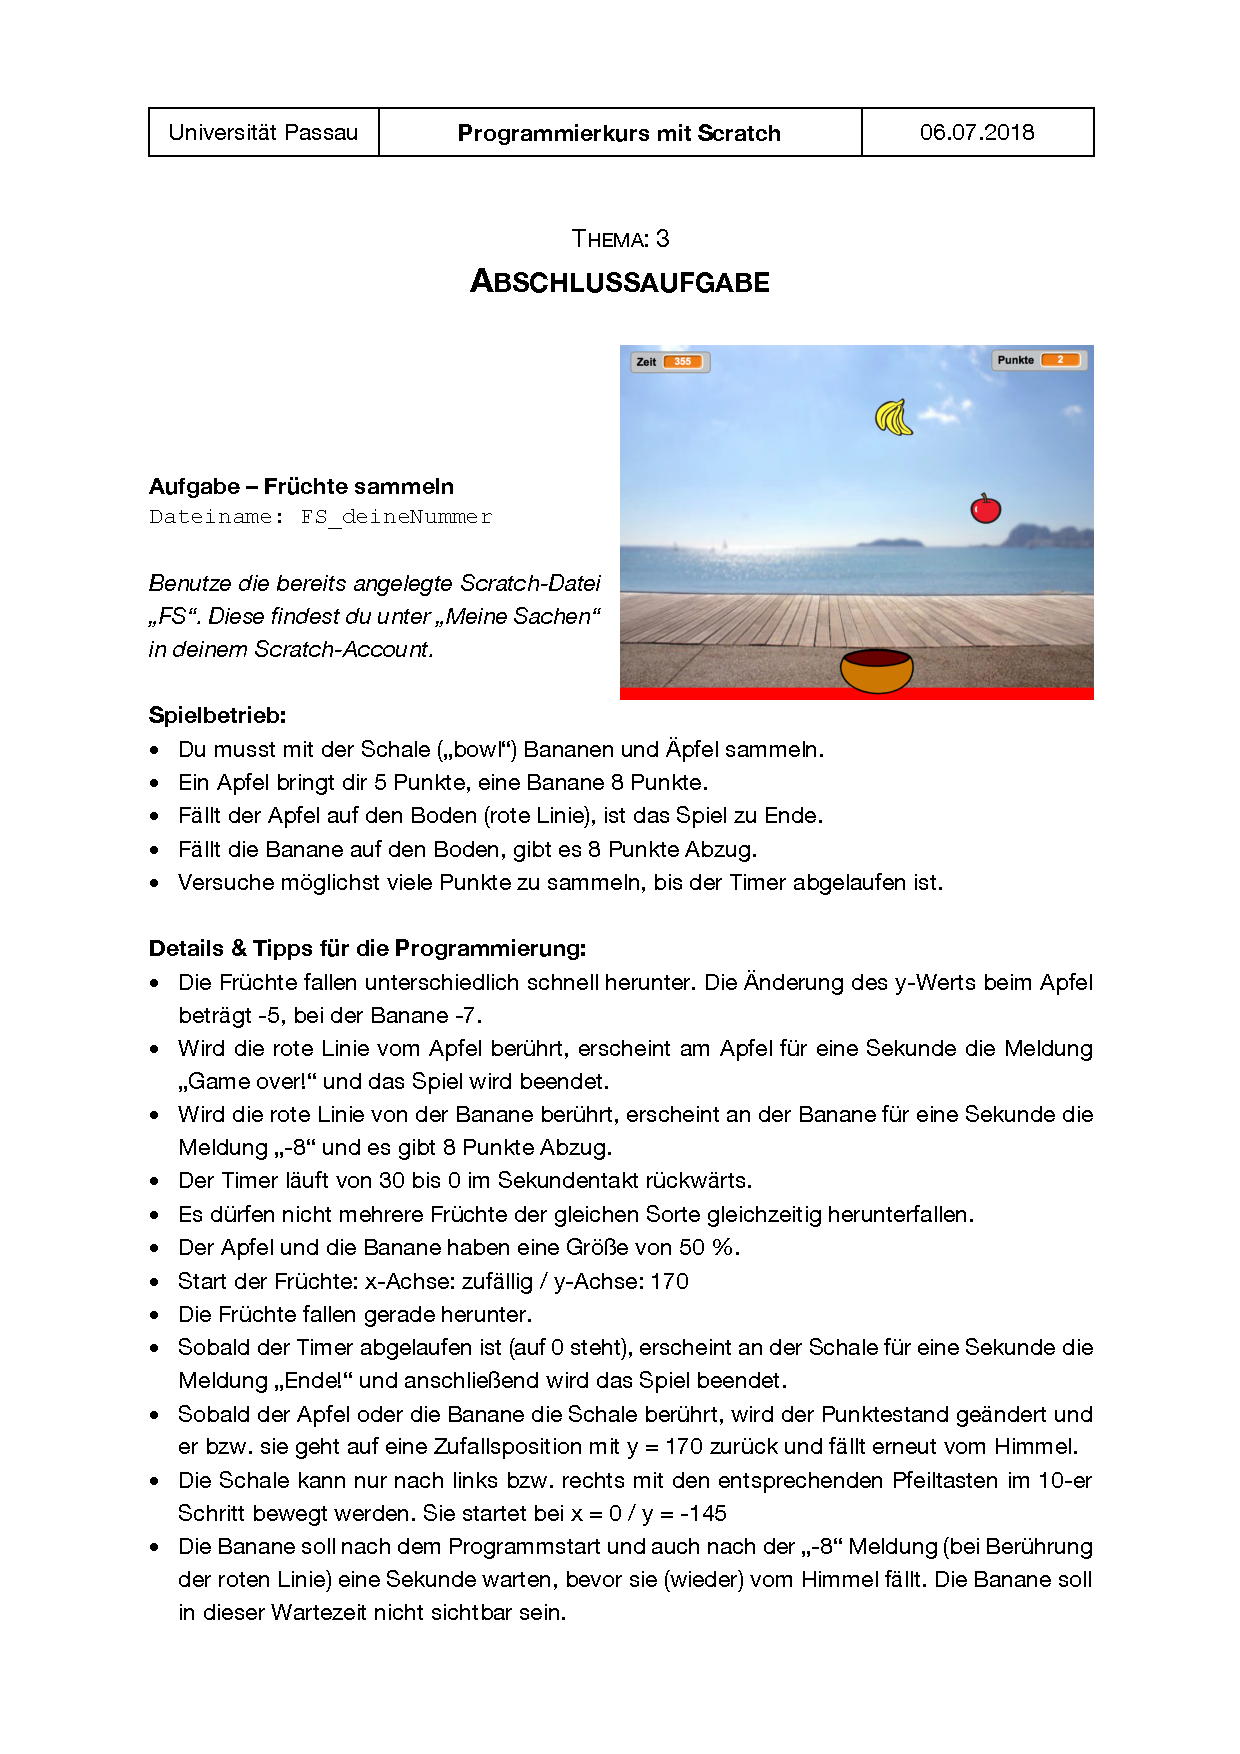
\includegraphics[width=\textwidth]{task-description}}
    \caption{Task description for the catching game (by Sebastian Keller \cite{keller})}
    \label{fig:catching_game_task_description}
\end{figure}


\section{Execution Time Evaluation}
\label{sec:time_measurement}

\begin{listing}
    \centering

    \begin{subfigure}[b]{.45\textwidth}
        \begin{minted}[autogobble, breaklines, linenos, fontsize=\tiny, framesep=2mm, frame=lines]{javascript}
            const names = [
                'callbacks-before',
                'random-inputs',
                'inputs',
                'sprites',
                'scratch',
                'callbacks-after',
                'constraints'
            ];

            let currentTimestamp;
            let currentRecord;
            let records;

            const resetRecords = function () {
                records = [];
            };

            const startRecord = function () {
                currentTimestamp = window.performance.now();
                currentRecord = [];
            };

            const record = function () {
                currentRecord.push(window.performance.now() - currentTimestamp);
            };

            const endRecord = function () {
                records.push(currentRecord);
            };

            const getRecords = function () {
                return {
                    names,
                    records
                };
            };
        \end{minted}
        \vspace{-\bigskipamount}
        \caption{Helper methods}
    \end{subfigure}
    \hspace{.08\textwidth}
    \begin{subfigure}[b]{.45\textwidth}
        \begin{minted}[autogobble, breaklines, linenos, fontsize=\tiny, framesep=2mm, frame=lines]{javascript}
            step () {
                startRecord();

                this.callbacks.callCallbacks(false);
                record();

                if (!this.running) {
                    endRecord();
                    return;
                }

                this.randomInputs.performRandomInput();
                record();

                this.inputs.performInputs();
                record();

                this.sprites.update();
                record();

                this.vm.runtime._step();
                record();

                if (!this.running) {
                    endRecord();
                    return;
                }

                this.callbacks.callCallbacks(true);
                record();

                if (!this.running) {
                    endRecord();
                    return;
                }

                const rv = this.constraints.checkConstraints();
                record();

                endRecord();

                return rv;
            }
        \end{minted}
        \vspace{-\bigskipamount}
        \caption{Modified step procedure}
    \end{subfigure}
    \caption{Modified Whisker step procedure for execution time measurement}
    \label{lst:time_measurement_code}
\end{listing}
